\documentclass{article}
\usepackage[utf8]{inputenc}
\usepackage[english]{babel}
\usepackage{graphicx}
\usepackage{pgfplots}
\begin{document}
\title{Usability of Web Browsers}
\author{Chris Dellomes\\
Professor: John Dionisio\\
CMSI 370: Interaction Design\\
	Loyola Marymount University}

\date{September 24, 2015}

\maketitle

\begin{center}
\begin{abstract}
\noindent This study is in response to the escalating competitive nature of the modern technology market. Usability is an ever growing factor in the success of software, necessitating usability tests. This paper presents comparative empirical evaluations involving two competing web browsers: Safari and Opera. Test participants were given three tasks to perform twice on each web browser. The results of this evaluation include (a) testing factors during the study, (b) quantitative data collected during testing, and (c) usability metrics measured. This paper incorporates the data gathered into a heuristic evaluation of each web browser.
\end{abstract}


\bigskip

\textit{Group Members}: Peyton Cross, Irakli Khizanishvili, Mary Reid
\end{center}

\thispagestyle{empty}

\clearpage

\setcounter{page}{1}

\section{Introduction} When Apple unveiled the Safari web browser back in 2003, it was advertised as the fastest web browser for the Macintosh and including a multitude of innovative features, such as a bookmark library. Originally exclusive to Apple computers, Safari later became available in 2007 for Windows until it was discontinued in 2012. Though not currently the most popular browser, it is currently the default web browser on iOS and OS X, with approximately 16\% of individuals globally using it as their preferred browser. Preceding Safari, Opera was originally a research project by Telenor until it became its own entity and publicly released in 1995. Users originally had to purchase Opera, until it moved to an advertisement based system which lasted from 2000 to 2005. Since its release, less than 5\% of web browser users worldwide used Opera as their preferred web browser, making it a relatively unpopular browser. While Safari is noticeably more widely used than Opera, they are comparable in terms of features.\\
\\
\indent Though neither browser is currently the most popular, it is still important to address the usability of each since Safari and Opera are still widely used worldwide. This study uses empirically examines the usability of each web browser. Within the Interaction Design field, usability is based on five distinct metrics: learnability, efficiency, errors, memorability, and satisfaction. This study will primarily focus on learnability, efficiency, and errors.

\section{Testing Factors} Before each test subject performed the assigned tasks, users were asked how much experience they had in using each web browser. Finding test subjects who had little to no prior experience with both web browsers was relatively simple. Since this study focused on both learnability and efficiency, we tested subjects when they were inexperienced with both browsers and again when they had ample experience performing the tasks.

\section{Testing Procedures} Each test subject performed three distinct tasks on each browser. They were tested when they had little to no experience to the browser, allowed to practice performing the tasks, then tested again once they felt comfortable performing the tasks.
\begin{enumerate}
	\item Change the home page of the web browser.
	\item Bookmark a webpage.
	\item Use the history to find and access a webpage visited the previous day.
\end{enumerate}
To keep the testing controlled, each subject was tested on a computer running OS X. As study participants performed each task, information regarding their learnability, efficiency, and errors were collected.

\subsection{Learnability}
\par
\textbf{First Task: } Change the home page of the web browser.
\begin{center}
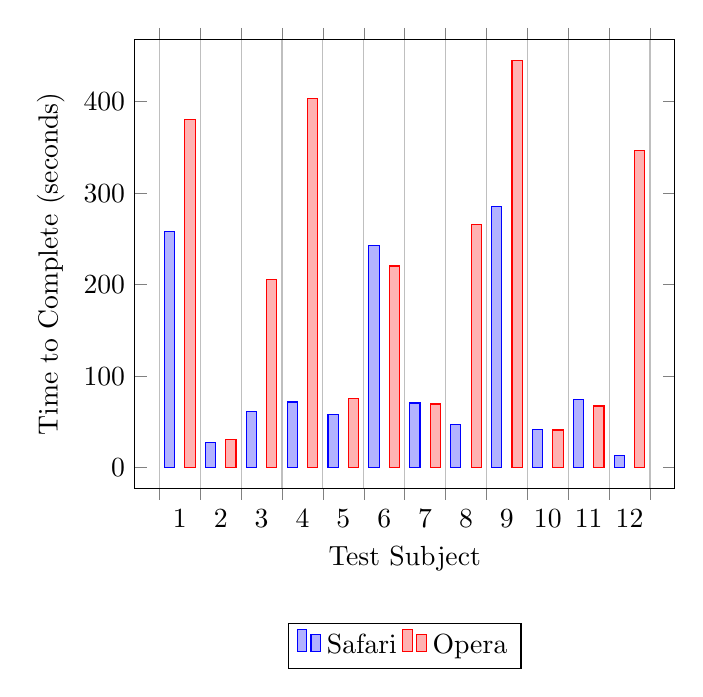
\begin{tikzpicture}
\begin{axis}[
	x tick label style={
		/pgf/number format/1000 sep=},
	xlabel= Test Subject,
	ylabel=Time to Complete (seconds),
	enlargelimits=0.05,
	legend style={at={(0.5,-0.3)},
	anchor=north,legend columns=-1},
	ybar interval=0.5,
]
\addplot 
	coordinates {(1, 258.1) (2, 27.6) (3, 61.5) (4, 71.8) (5, 57.8) (6, 243.0) (7, 70.7) (8, 46.8) (9, 285.2) (10, 41.7) (11, 74.9) (12, 13.1) (13, 0)};
\addplot
	coordinates {(1, 381.0) (2, 30.7) (3, 205.7) (4, 403.0) (5, 75.6) (6, 220.4) (7, 69.6) (8, 265.4) (9, 445.4) (10, 41.2) (11, 67.4) (12, 346.2) (13, 0)};
\legend{Safari,Opera}
\end{axis}
\end{tikzpicture}

\par Average time for Learnability task \#1 on Safari: \textit{104.4 seconds}
\par Average time for Learnability task \#1 on Opera: \textit{212.6 seconds}
\end{center}
\par \noindent The results of this task indicate that on average, it is significantly easier to learn how to change the home page in Safari.

\clearpage

\par
\textbf{Second Task: } Bookmark a webpage.
\begin{center}
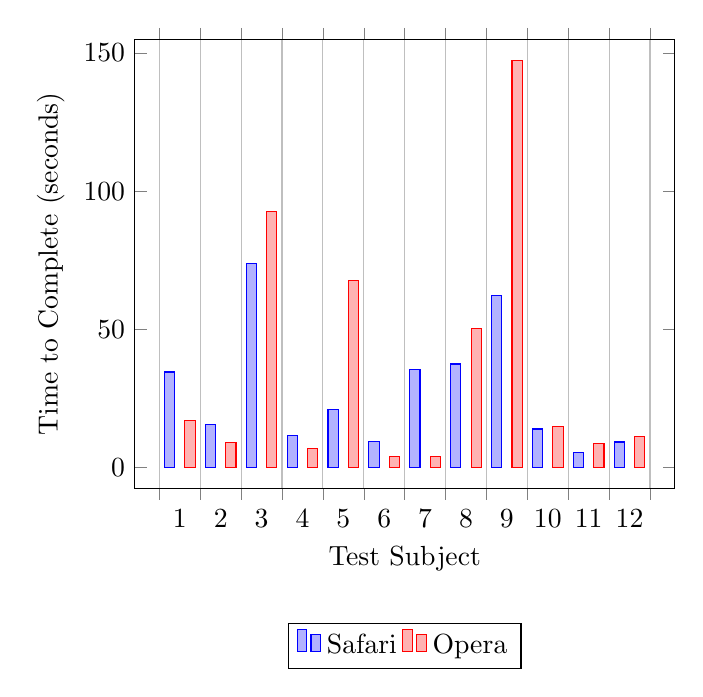
\begin{tikzpicture}
\begin{axis}[
	x tick label style={
		/pgf/number format/1000 sep=},
	xlabel= Test Subject,
	ylabel=Time to Complete (seconds),
	enlargelimits=0.05,
	legend style={at={(0.5,-0.3)},
	anchor=north,legend columns=-1},
	ybar interval=0.5,
]
\addplot 
	coordinates {(1, 34.6) (2, 15.6) (3, 73.7) (4, 11.7) (5, 21.2) (6, 9.4) (7, 35.4) (8, 37.5) (9, 62.2) (10, 14.0) (11, 5.6) (12, 9.3) (13, 0)};
\addplot
	coordinates {(1, 17.1) (2, 9.1) (3, 92.8) (4, 6.8) (5, 67.7) (6, 3.9) (7, 4.0) (8, 50.2) (9, 147.4) (10, 14.9) (11, 8.8) (12, 11.2) (13, 0)};
\legend{Safari,Opera}
\end{axis}
\end{tikzpicture}

\par Average time for Learnability task \#1 on Safari: \textit{27.5 seconds}
\par Average time for Learnability task \#1 on Opera: \textit{36.2 seconds}
\end{center}
\par \noindent The results of this task indicate that on average, it is easier to learn how to bookmark a page in Safari.

\clearpage

\par
\textbf{Third Task: } Use the history to find and access a webpage visited the previous day.
\begin{center}
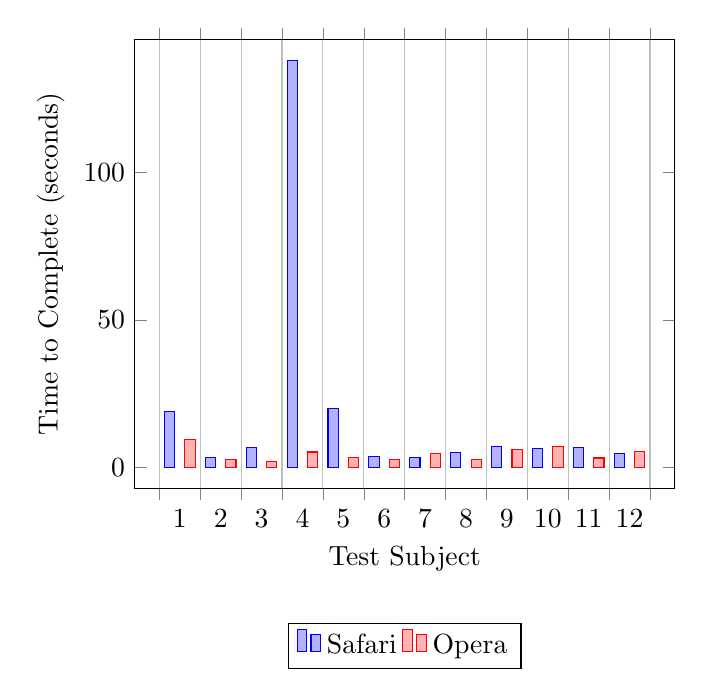
\begin{tikzpicture}
\begin{axis}[
	x tick label style={
		/pgf/number format/1000 sep=},
	xlabel= Test Subject,
	ylabel=Time to Complete (seconds),
	enlargelimits=0.05,
	legend style={at={(0.5,-0.3)},
	anchor=north,legend columns=-1},
	ybar interval=0.5,
]
\addplot 
	coordinates {(1, 19.1) (2, 3.5) (3, 6.8) (4, 138.0) (5, 20.1) (6, 3.9) (7, 3.5) (8, 5.2) (9, 7.1) (10, 6.5) (11, 6.9) (12, 4.9) (13, 0)};
\addplot
	coordinates {(1, 9.7) (2, 2.8) (3, 2.2) (4, 5.3) (5, 3.5) (6, 2.7) (7, 4.9) (8, 2.7) (9, 6.3) (10, 7.3) (11, 3.3) (12, 5.4) (13, 0)};
\legend{Safari,Opera}
\end{axis}
\end{tikzpicture}

\par Average time for Learnability task \#1 on Safari: \textit{18.8 seconds}
\par Average time for Learnability task \#1 on Opera: \textit{5.3 seconds}
\end{center}
\par \noindent The results of this task indicate that on average, it is easier to learn how to access the histoey in Opera.

\clearpage

\subsection{Efficiency}
\par
\textbf{First Task: } Change the home page of the web browser.

\par
\textbf{Second Task: } Bookmark a webpage.

\par
\textbf{Third Task: } Use the history to find and access a webpage visited the previous day.

\end{document}